\section{Durchführung}
\label{sec:Durchführung}

\begin{figure}
  \centering
  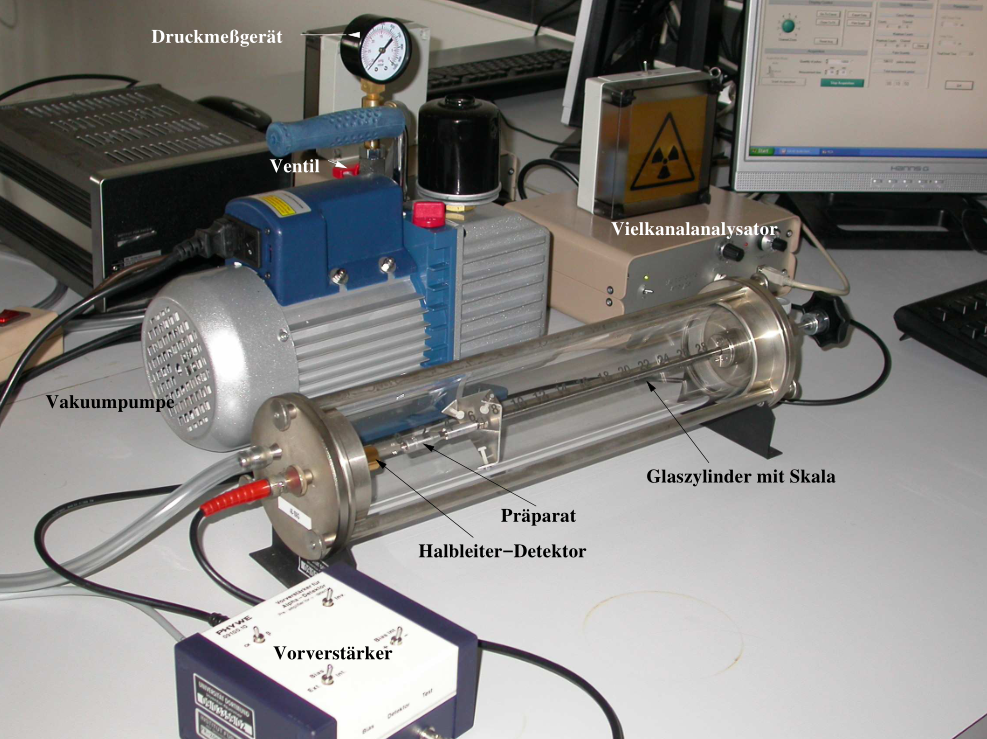
\includegraphics{data/abb1.png}
  \caption{Aufbau zur Bestimmung der Reichweite von \alpha-Strahlung.}
  \label{fig:abbA1}
\end{figure}
\FloatBarrier

In einem evakuierbaren Glaszylinder befinden sich ein α-Präparat und ein Detektor. 
Als Strahlungsquelle dient ein Am-Präparat, das mit einer Halbwertzeit $T_{1/2} = 458$ a entsprechend
\begin{equation}
    _{95}^{241}\text{Am} \longrightarrow _{93}^{237}\text{Np} + _{2}^{4}\text{He}^{++}
    \label{eqn:gl4}
\end{equation}
zerfällt.
Durch den verschiebbaren Halter des $\alpha$-Strahlersist der Abstand zwischen diesem und dem Detektor variabel.
Der gemessene Puls des Halbleiter-Sperrschichtzählers wird mit einem Vorverstärker vertärkt und in einem Vielkanalanalysator entsprechend seiner Pulshöhe analysiert.
Die Energie der $\alpha$-Teilchen ist proportional zur Pulshöhe und kann in Form eines Histogramms aufgenommen werden.
Vor dem Beginn der Messung müssen  die Diskreminatorschwellen am Vielkanalanalysator eingestellt werden.
Dazu wird der Abstand Quelle-Detektor so maximiert, dass der Multichannal Analyzer gerade anfängt zu zählen.

\subsection{Reichweite von \alpha-Strahlung}
Bei einem Druck von $p = 0$ mbar wird die Messung begonnen.
Dann wird der Druck Schrittweise in 50 mbar Schritten erhöht, bei einer Messzeit von mindestens 120 s.
Es wird das Energiemaximum und die Gesamtzählrate notiert.
Wenn von einer linearen Energieskala ausgegangen wird kann hierdurch die Energie als Funktion des Drucks bestimmt werden.
